\subsection{Serial Port}
\label{sec:serial_port}

The serial port in the DE2-115 Computer implements a UART that is connected to an RS232
chip on the \DEBoard~board.  This UART is configured for 8-bit data, one stop bit, odd parity, and
operates at a baud rate of 115,200.  The serial port's programming interface 
consists of two 32-bit registers, as illustrated in Figure \ref{fig:serial_port}. 
The register at address {\sf 0xFF201010} is referred to as the
{\it Data} register, and the register at address {\sf 0xFF201014} is called the {\it
Control} register.

\begin{figure}[h!]
   \begin{center}
       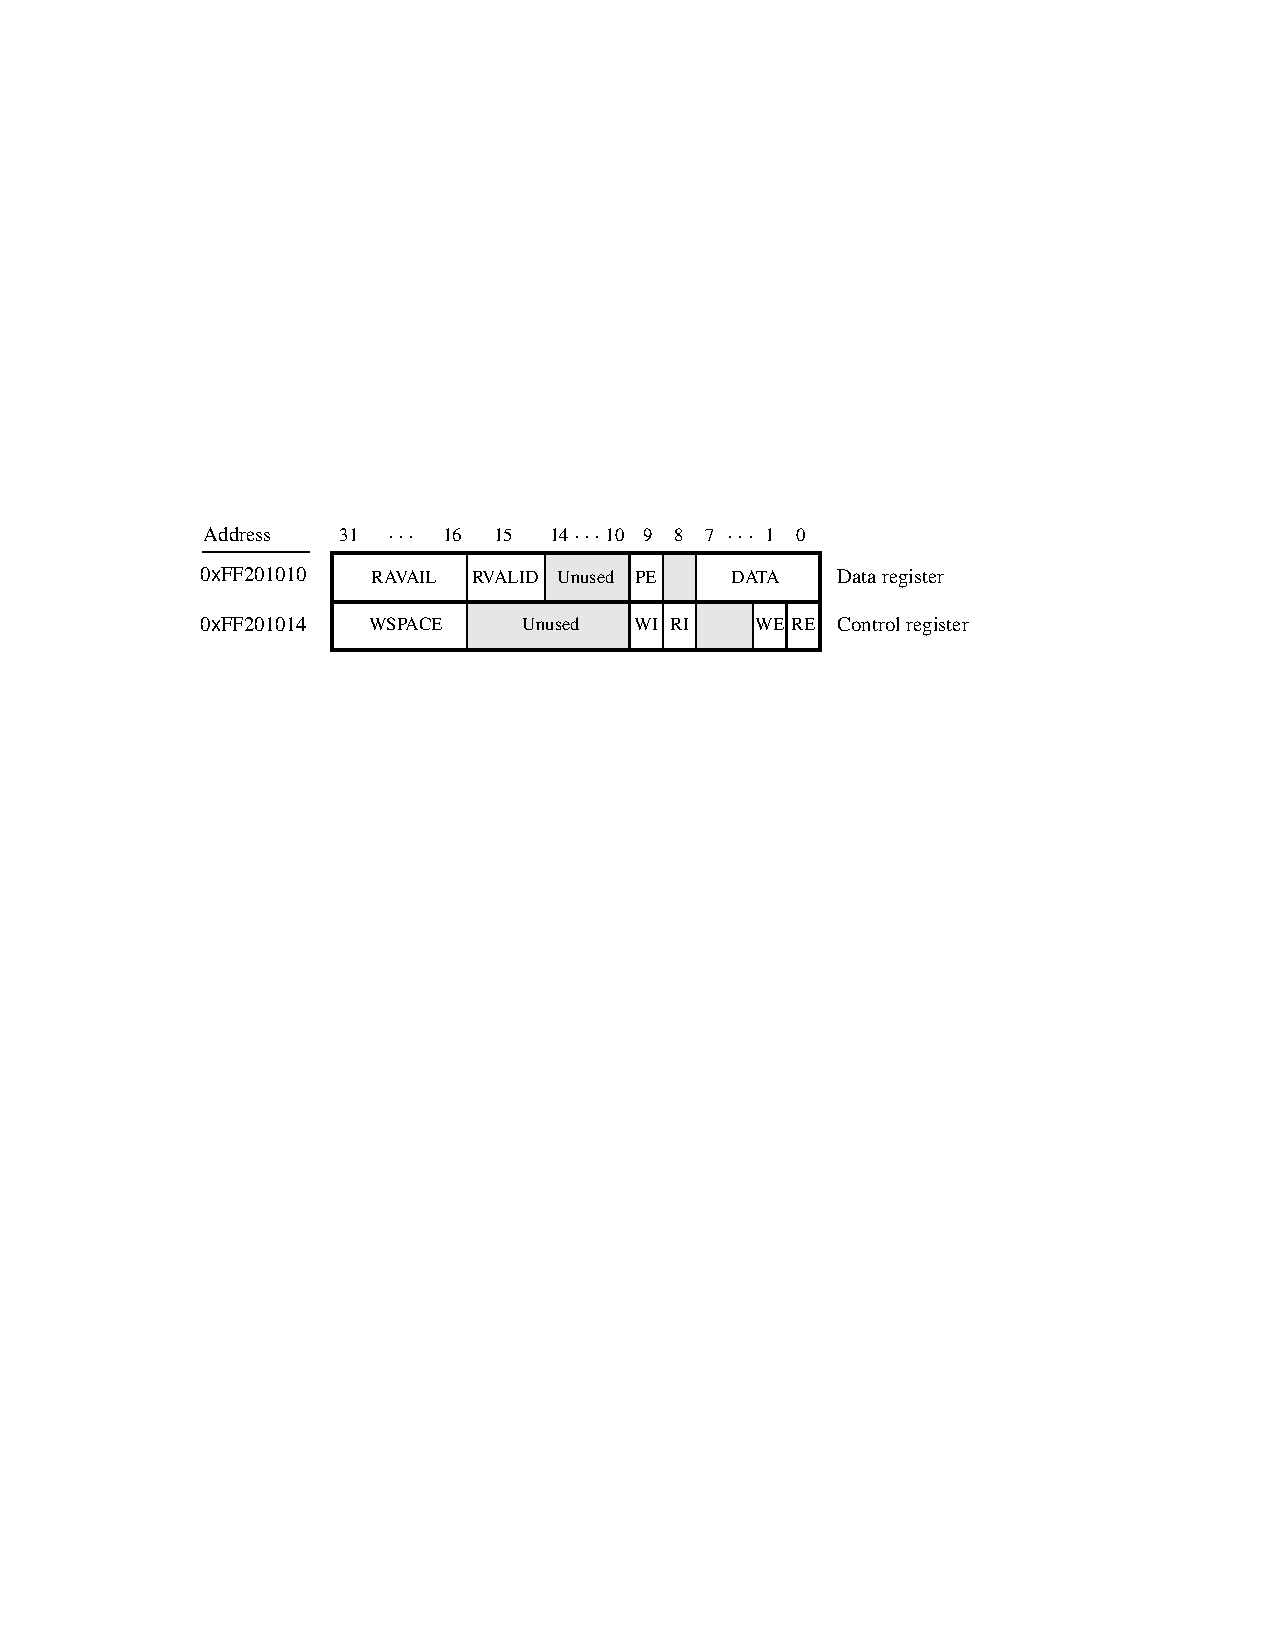
\includegraphics{../../../common/figs/Media_FPGA_Serial.pdf}
   \end{center}
   \caption{Serial port UART registers.}
	\label{fig:serial_port}
\end{figure}

When character data is received from the RS 232 chip it is stored in a 256-character
FIFO in the UART. As illustrated in Figure \ref{fig:serial_port}, the number 
of characters, {\it RAVAIL}, currently stored in this FIFO is
provided in bits 31$-$16 of the {\it Data} register.  If the receive FIFO overflows, then
additional data is lost.  When the data that is present in the receive FIFO is available 
for reading, then the value of bit 15, {\it RVALID}, will be 1. Reading the character at
the head of the FIFO, which is provided in bits $7-0$, decrements the value of {\it RAVAIL} 
by one and returns this decremented value as part of the read
operation. If no data is available to be read from the receive FIFO, then {\it RVALID} will 
be set to 0 and the data in bits $7-0$ is undefined.

The UART also includes a 256-character FIFO that stores data waiting to be sent to the RS 232
chip. Character data is loaded into this FIFO by performing a write to bits 7$-$0
of the {\it Data} register.  Writing into this register has no effect 
on received data.  The amount of space, {\it WSPACE}, currently available in the transmit FIFO is 
provided in bits 31$-$16 of the {\it Control} register, as indicated 
in Figure \ref{fig:serial_port}.  If
the transmit FIFO is full, then any additional characters written to the {\it Data} 
register will be lost.

The {\it Control} register bits {\it RE}, {\it WE}, {\it RI}, and {\it WI} are described 
in section \ref{sec:exceptions}.